\pdfbookmark[1]{jj}{jj}
\chapter{Josephson junctions}\label{chap:jj}



\section{Superconductivity}
    \begin{figure}
        \centering
        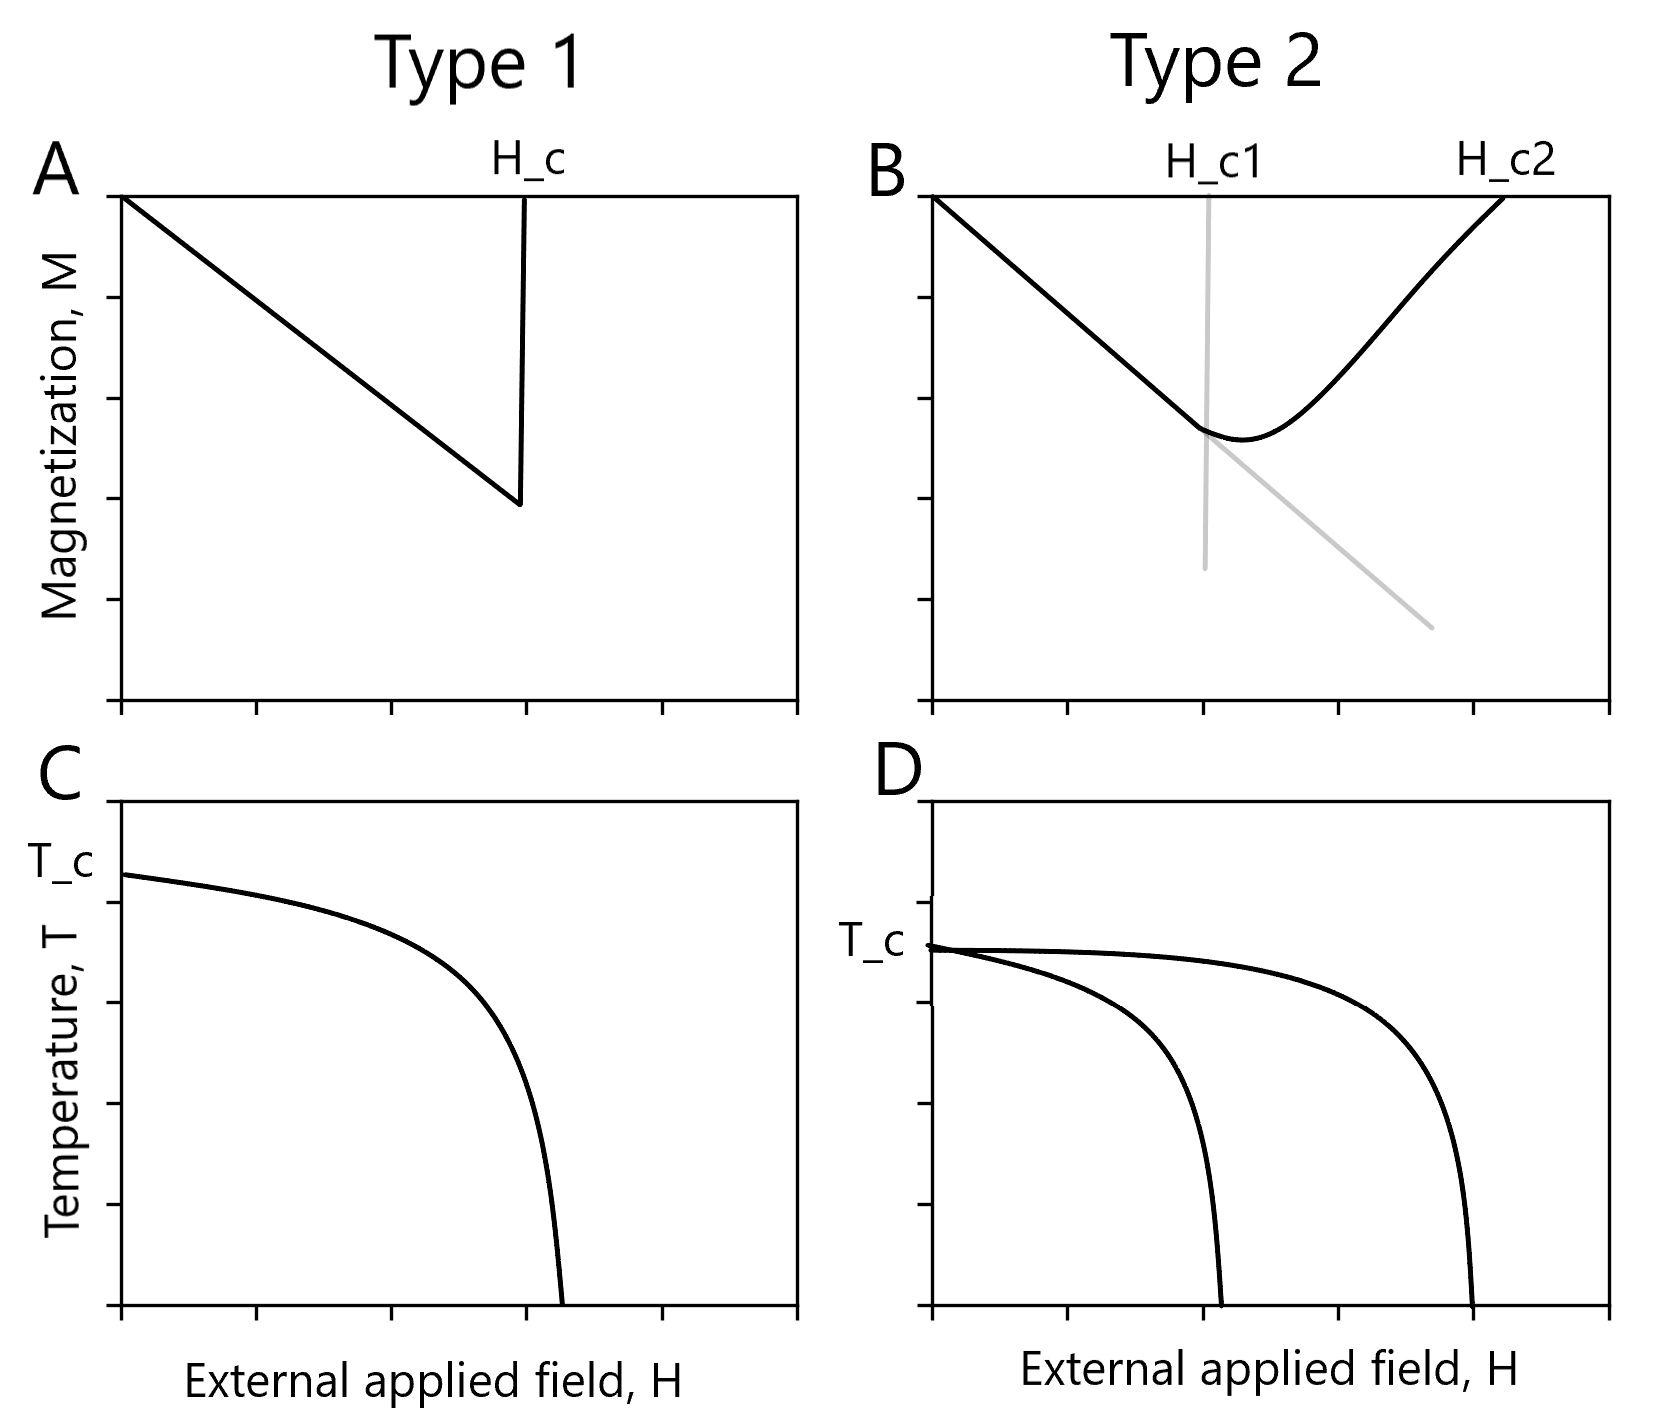
\includegraphics[width = 13cm]{Images/critical field.png}
        \caption[Type 1 and type 2 superconductor]{\textbf{Type 1 and type 2 superconductor:} A) Type 1 superconductor. $H_c$ is the critical field where the magnetization gets destroyed. instantaneously. B) Type 2 superconductor have two critical fields, $H_{c1}$ and $H_{c2}$. At $H_{c1}$, some flux-lines start to be able to enter the superconductor. At $H_{c2}$, the superconductivity is destroyed and the superconductor don't produce a magnetization anymore. C) and D) the critical temperature $T_c$ as a function of the external magnetic field applied.}
        \label{fig:type1and2}
    \end{figure}
    A superconductor is a material in which you can prove the Meissner–Ochsenfeld effect below a critical temperature, $T_c$, or at very high pressures. The Meissner effect is a property of thermal equilibrium and states that a weak external magnetic field will be expelled by a superconductor below $T_c$ independently of how it was cooled down. In order for the superconductor to repel the small external magnetic field, $\Vec{B}_{ext}$, it must produce an equal but opposite magnetization \cite{Annett2004}: 
    \begin{equation}
        \Vec{B}_{ext}=\mu_0 (\Vec{H}_{ext} + \Vec{M}) = 0 \Leftrightarrow \Vec{H}_{ext} = - \Vec{M}
    \end{equation}
    The magnetic susceptibility is then given by: 
    \begin{equation}
        \chi=\left.\frac{d M}{d H}\right|_{\lim_{H\to 0}}= -1
    \end{equation}
    This tells us the superconductor is a diamagnet and since it completely repels the external field, it is said to be a perfect diamagnet. However, this is only true for small external fields. When the strength of the field increases, two possible things can happen dependent on, if the superconductor is type 1 or type 2. A type 1 superconductor will repel the external magnetic field until a critical field, $H_{c}$. At this field, the superconductivity is abruptly destroyed and the magnetization, $\Vec{M}$ goes to 0 instantaneously as seen in fig. \ref{fig:type1and2} A). A type 2 superconductor exhibit a change in behavior at two critical fields, $H_{c1}$ and $H_{c2}$. At $H_{c1}$, some flux-lines start to be able to enter the superconductor. The amount of flux-lines which can enter, will increase linearly between $H_{c1}$ and $H_{c2}$ as a function of $H$. At $H_{c2}$, the superconductivity is destroyed and the superconductor don't produce a magnetization anymore as seen in fig. \ref{fig:type1and2} B. The critical fields for which both type 1 and type 2 superconductors change behavior, is itself a function on temperature. This is seen in fig. \ref{fig:type1and2} B) and C). At $T_c$ the superconductors undergo a 2nd order phase transition from a "superconductor" to a "normal metal". Since we are only interested in the superconducting properties, we will from now on only assume temperatures below $T_c$. 
    \newline
    \newline
    Besides, from the magnetic properties of superconductors, they are also shown to posses persistent current meaning it can carry a current without an external energy source. The persistent current is due to the fact, that superconductors exhibit zero resistivity, $\rho = 0 $, and can therefore carry a flow of electrons without getting scattered into phonons or other electrons. The relationship between the super current density and the magnetic vector potential is given by the London equation \cite{Annett2004}:
    \begin{equation}
        \Vec{j}_s=-\frac{n_s e^2}{m_e} \Vec{A}
    \end{equation}
    The current running in superconductors is due to cooper pairs which are pairs of electrons. The cooper pairs and the critical temperature can be described by the Bardeen–Cooper–Schrieffer theory, \acrshort{bcs} theory. The \acrshort{bcs} theory is a microscopic quantum theory of superconductivity and is described in the following section in order to better understand why electrons forms cooper pairs and what conditions should be fulfilled in doing so. 
  
    \subsection{Mean field BCS theory and cooper pairs}
         The formation of cooper pairs is due to an attractive potential between 2 electrons close to the Fermi surface. Electrons interact via a phonon where the effective potential is given by \cite{Annett2004}: 
          \begin{equation}
            V_{\mathrm{eff}}{q}, \omega)=\left|g_{\mathrm{eff}}\right|^2 \frac{1}{\omega^2-\omega_D^2}
        \end{equation}
        If $|\omega < \omega_D|$, the effective potential is attractive. Therefore, it is only electrons which have energies within $\varepsilon_f \pm \hbar \omega_D$ which participate in forming cooper pairs. Assuming all states up to the fermi wave vector, $k_f$, is filled. Adding 2 electrons within $\varepsilon_f +\hbar \omega_D$ will create a cooper pair. The 2 particle wave function is anti symmetric and can be divided into two parts, a spacial- and a spin wave function: 
        \begin{equation}
            \Psi(r_1,r_2,\sigma_1,\sigma_2) = e^{i\Vec{k}\Vec{r}} \varphi(r_1-r_2) \phi^{spin}_{\sigma_1,\sigma_2}
        \end{equation}
        Due to anti symmetry of Fermions, we know that the position and spin wave function should have opposite symmetry. The lowest energetic configuration is when the cooper pairs have opposite k-vector and therefore $\Vec{k}=0$. Further, the position wave function: $\varphi\left(\mathbf{r}_1-\mathbf{r}_2\right) = + \varphi\left(\mathbf{r}_2-\mathbf{r}_1\right)$ is an even function. Therefore, $\phi^{spin}_{\sigma_1,\sigma_2} = \frac{1}{\sqrt{2} }|\uparrow \downarrow \rangle - |\downarrow \uparrow \rangle $ is an uneven function and it turns out that it is in a singlet state \cite{Annett2004}.
        \newline
        \newline
        The  Hamiltonian for describing the electron-electron interaction for opposite spin, $\sigma_1=-\sigma_2$,  and opposite k vector, $k_1=-k_2$ is given by\cite{Annett2004}: 
        \begin{equation}\label{Hamiltonian_BCS}
            \hat{H}=\sum_{\mathbf{k}, \sigma} (\varepsilon_{\mathbf{k}}-\mu) c_{\mathbf{k} \sigma}^{\dagger} c_{\mathbf{k} \sigma}-\left|g_{eff}\right|^2 \sum_{\mathbf{k} \mathbf{k'}} c_{\mathbf{k}_{\uparrow}}^{\dagger} c_{-\mathbf{k}_{\downarrow}}^{\dagger} c_{\mathbf{k'}_{\downarrow}} c_{\mathbf{k'}_{\uparrow}} 
        \end{equation}
        The first term is the self energy of an electron and the second term is the electron-electron interaction. The $c$ and $c^{\dagger}$ is the operators which change the occupation number of the Fock space.
        \begin{equation}
            c^{\dagger}|0\rangle = |1\rangle, c |1\rangle = |0 \rangle
        \end{equation}
        We use a mean field approximation and the Bogoliubov-Valentin transformation and rewrite the Hamiltonian as: 
        \begin{equation}
        \hat{H}_{MF}= \sum_{\mathbf{k} ,\sigma} (\varepsilon_{\mathbf{k}}-\mu) c_{\mathbf{k} \sigma}^{\dagger} c_{\mathbf{k} \sigma}-\left|g_{eff} \right|^2 \sum_{\mathbf{k} \mathbf{k'}} \left(\langle c_{\mathbf{k_{\uparrow}}}^{\dagger} c_{-\mathbf{k} \downarrow}^{\dagger}\rangle c_{-\mathbf{k}^{\prime}_{\downarrow} }c_{\mathbf{k}^{\prime}_{\uparrow}} + c_{\mathbf{k}_{\uparrow}}^{\dagger} c_{-\mathbf{k}_{\downarrow}}^{\dagger} \langle c_{-\mathbf{k'}_{\downarrow}} c_{\mathbf{k'_{\uparrow}}} \rangle \right)
        \end{equation}
        Due to symmetry of our occupation number operators, this  can be rewritten into: 
        \begin{equation}
            \hat{H}_{MF}=\sum_{\mathbf{k} \sigma}\left(\varepsilon_{\mathbf{k}}-\mu\right) c_{\mathbf{k} \sigma}^{\dagger} c_{\mathbf{k} \sigma}-\sum_{\mathbf{k}}\left(\Delta^* c_{-\mathbf{k} \downarrow} c_{\mathbf{k} \uparrow}+\Delta c_{\mathbf{k} \uparrow}^{\dagger} c_{-\mathbf{k} \downarrow}^{\dagger}\right)
        \end{equation}
        Where $\Delta$ is defined as: 
        \begin{equation}
            \Delta = \left|g_{eff} \right|^2 \sum_{\mathbf{k}} \langle c_{-\mathbf{k'}_{\downarrow}} c_{\mathbf{k'_{\uparrow}}} \rangle
        \end{equation}
        We can now write the Hamiltonian in the form of a matrix: 
        \begin{equation}
            \hat{H}_{MF}=\sum_{\mathbf{k}}\left(\begin{array}{ll}
            c_{\mathbf{k} \uparrow}^{\dagger} & c_{-\mathbf{k} \downarrow}
            \end{array}\right)\left(\begin{array}{cc}
            \varepsilon_{\mathbf{k}}-\mu & -\Delta \\
            -\Delta^* & -\left(\varepsilon_{\mathbf{k}}-\mu\right)
            \end{array}\right)\left(\begin{array}{c}
            c_{\mathbf{k} \uparrow} \\
            c_{-\mathbf{k} \downarrow}^{\dagger}
            \end{array}\right)
        \end{equation}
        The eigen energies of the square matrix is $E_k = \sqrt{(\varepsilon_k-\mu)} + |\Delta|^2$. The relationship between $\Delta$ and $E_k$ is very important as it tell us how an incoming electron into a superconductor behave and thereby the energy needed to create a cooper pair. We call $\Delta$ our order parameter and it determines if we are in the normal state (above $T_c$, $\Delta = 0$) or in the superconducting state (below $T_c$, $\Delta \neq 0$). In the superconducting state, the energy associated with adding an electron is $+E_k$. The minimum energy associated for making an excitation is $2\Delta$ which is the energy gap of the superconductor. Electrons going into the superconductor must therefore posses energy $E_k > \Delta$  which is why it can be related to the binding energy of creating a cooper pair.
        
    \subsection{Josephson tunnel junction}
        \begin{figure}
            \centering
                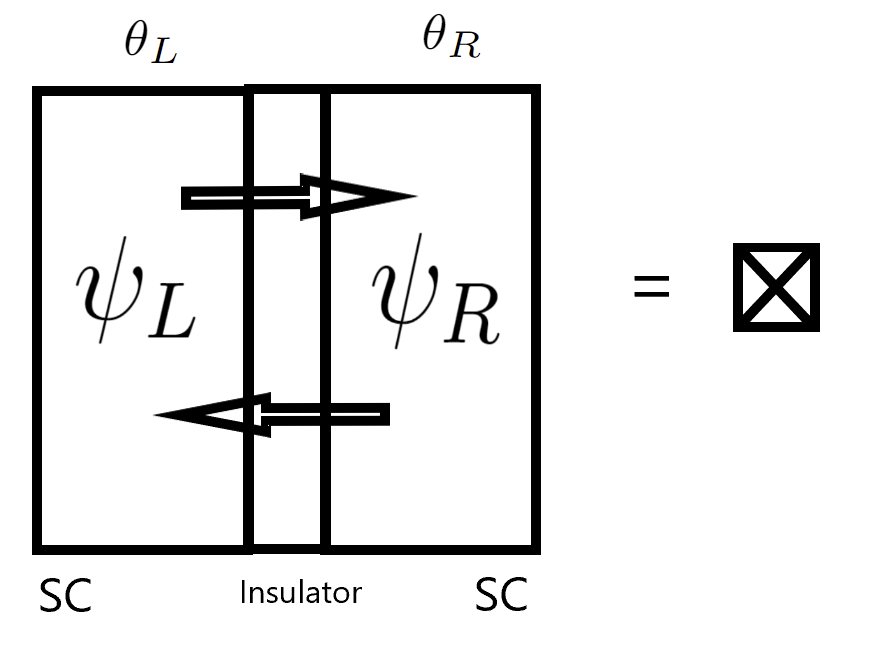
\includegraphics[width = 10cm]{Images/Josephson junction.png}
                \caption[Schematic drawing of a Josephson Junction]{\textbf{Schematic drawing of a Josephson junction:} The $\theta_L$ and $\theta_R$ is the phase of each superconductors. The $\psi_L$($\psi_R$) is the macroscopic wave functions describing the cooper pairs on the left(right) superconductor.}
            \label{fig:JJ}
        \end{figure}
        A Josephson junction is an electrical component consisting of 2 superconductors separated by an insulating layer as seen in \ref{fig:JJ}. The Josephson junction allows the tunneling of cooper pairs between the two superconductors through the insulating layer. This tunneling effect is called the Josephson effect. It can be described mathematically because the states of the cooper pairs on each superconductor can be described by a coherent wave function $\psi_0$ which posses  Off Diagonal Long Range Order, \acrshort{odlro}. \acrshort{odlro} can be physical interpreted as the coherent wave function describing cooper pairs (pairs of electrons) is valid even though the cooper pairs are very far away. By using the macroscopic wave function to describe the cooper pairs on each side, the hamiltonian for describing the whole system becomes: 
        \begin{equation}
        \hat{H} = 
            \begin{bmatrix}
            \frac{2eV}{2} & T \\
            T & -\frac{2eV}{2} 
            \end{bmatrix} 
        \end{equation}
        Where the $2e$ is from the charge of the 2 cooper pairs and $ \pm \frac{V}{2}$ is the voltage lifted(lower) the potential in the side. The $T$ is the transmission term which says how easily the cooper pairs are able to tunnel through the insulating layer. $T$ is dependent on the thickness and materials of the insulating layer. Inserting the Hamiltonian into the Schrodinger equation will give the following equations: 
        \begin{equation}
                \frac{d \Psi}{d t} 
            =
                \frac{1}{i \hbar}\hat{H}\Psi
            \Rightarrow
                \begin{bmatrix}
                    \frac{d \psi_L}{dt} \\
                    \frac{d \psi_R}{dt} 
                \end{bmatrix}  
            =    
                \frac{1}{i \hbar} 
                \begin{bmatrix}
                \psi_L e V + \psi_R T \\
                \psi_L T - \psi_R e V  
                \end{bmatrix}
        \end{equation}
        The current from one side to the other in the Josephson junction is given by the change in number of cooper pairs in one superconductor over time multiplied with the charge of the cooper pairs: 
        \begin{equation}
            \begin{aligned}
                I_L &= -I_R =  \frac{d|\psi_L|}{dt} 2e = 2e \left( \Dot{\psi}_L^* \psi_L + \psi_L^* \Dot{\psi_L} \right) \Rightarrow 
                \\
                I_L &= \frac{2e}{i\hbar} \left( -eV |\psi_L|^2 - \psi_R^*\psi_L + e V  |\psi_L|^2 + T \psi_L^*\psi_R \right) 
            \end{aligned}
        \end{equation}
        Using that $\psi_{L(R)} = Re(\psi_{L(R)}) + i Im(\psi_{L(R)})$ and $\psi_{L(R)}^* = Re(\psi_{L(R)}) - i Im(\psi_{L(R)})$, we obtain that only the imaginary part is left: 
        \begin{equation}
            I_L = \frac{4 e T}{\hbar} Im(\psi^*_L \psi_R)
        \end{equation}
        Assuming that the transmission, $T$, is small, we can approximate the off diagonal terms in the Hamiltonian as a small perturbation to a system with no transmission of cooper pairs, $\mathring{\Psi}$. 
        \begin{equation}
            \begin{aligned}
                 I_L &= \frac{4 e T}{\hbar} Im(\mathring{\psi}^*_L \mathring{\psi}_R) + \text{small perturbation} \\
                    \mathring{\psi}^*_L &= |\mathring{\psi}_L| e^{(i V e)/\hbar t - i\theta_L}\\
                    \mathring{\psi}_R &= |\mathring{\psi}_R| e^{(i V e)/\hbar t + i\theta_R}
            \end{aligned}
        \end{equation}
        \begin{equation} \label{eq:JJ1}
            \Rightarrow I_L = I_c sin(\Delta \theta)
        \end{equation}
        Where $\Delta \theta = \theta_R- \theta_L$ is the difference in phase between the 2 superconductors and $I_c = \frac{4 e T }{\hbar}$ is the critical current dependent on the geometry and material of the insulating layer. The critical current is the max current the copper pairs can make. Currents $I< I_L$ are dissipationless and are often referred to as a super current $I_S = I_L $.  The eq. \ref{eq:JJ1} is called the first Josephson equation and tells us that the supercurrent, $I_s$ is proportional to to the phase difference between the two superconductors. The other Josephson equation is given by: 
        \begin{equation}
            \begin{aligned}
                \frac{\partial\Delta \theta}{\partial t } &= \frac{2e}{\hbar} V(t) \\
                V(t) &= \frac{\partial \Delta \theta}{\partial t} \frac{\hbar }{2 e}
            \end{aligned}
        \end{equation}
        Which gives us a relation between the change in phase and the voltage applied. When a current runs through the Josephson junction, there will be stored an energy depended on the phase difference between the two superconductors, $\Delta \theta$. The energy is given by \cite{Krantz2019}:
        \begin{equation}
            E(\Delta \theta) = -E_J cos(\Delta \theta) 
        \end{equation}
        Where $E_J =  \frac{\Psi_0 I_c}{2 \pi}$. From now on, we will write $\Delta\theta = \phi$. 
        Some text where you end up with the hamiltonian as we show in 
        \begin{equation}
            Josephson:& \quad h_{J} = E_j \cos \left(\frac{\Phi 2 \pi}{\Phi_0} \right)    \\
        \end{equation}

    \subsection{Manhattan style junction}